\qrchapter{https://forgottenpillar.com/rsc/en-fp-chapter11}{The personality of God - by James S. White}


\qrchapter{https://forgottenpillar.com/rsc/en-fp-chapter11}{شخصانية الله - بقلم جيمس س. وايت}


In what follows, we will examine James White’s pamphlet titled “\textit{The Personality of God}”. When we read this article, we will see that James White continues where Brother Loughborough left off, and that he expands and deepens the understanding behind the first point of the \emcap{Fundamental Principles}.


فيما يلي، سنفحص كتيب جيمس وايت بعنوان “\textit{شخصانية الله}”. عندما نقرأ هذه المقالة، سنرى أن جيمس وايت يواصل من حيث انتهى الأخ لوبورو، وأنه يوسع ويعمق الفهم وراء النقطة الأولى من \emcap{المبادئ الأساسية}.


James White’s tract was printed multiple times, advertised 54 times, and reprinted twice in the Review and Herald publication. His view on the \emcap{personality of God} was well known and spread throughout Adventism. In this pamphlet, we will see clear criticism toward the ideas that Kellogg advocated in the Living Temple.


تمت طباعة نشرة جيمس وايت عدة مرات، وتم الإعلان عنها 54 مرة، وأعيد طباعتها مرتين في مجلة ريفيو آند هيرالد. كانت وجهة نظره حول \emcap{شخصانية الله} معروفة جيدًا ومنتشرة في جميع أنحاء الأدفنتزم. في هذا الكتيب، سنرى نقدًا واضحًا للأفكار التي دافع عنها كيلوغ في كتاب ذا ليفينغ تمبل.


\begin{figure}[hp]
    \centering
    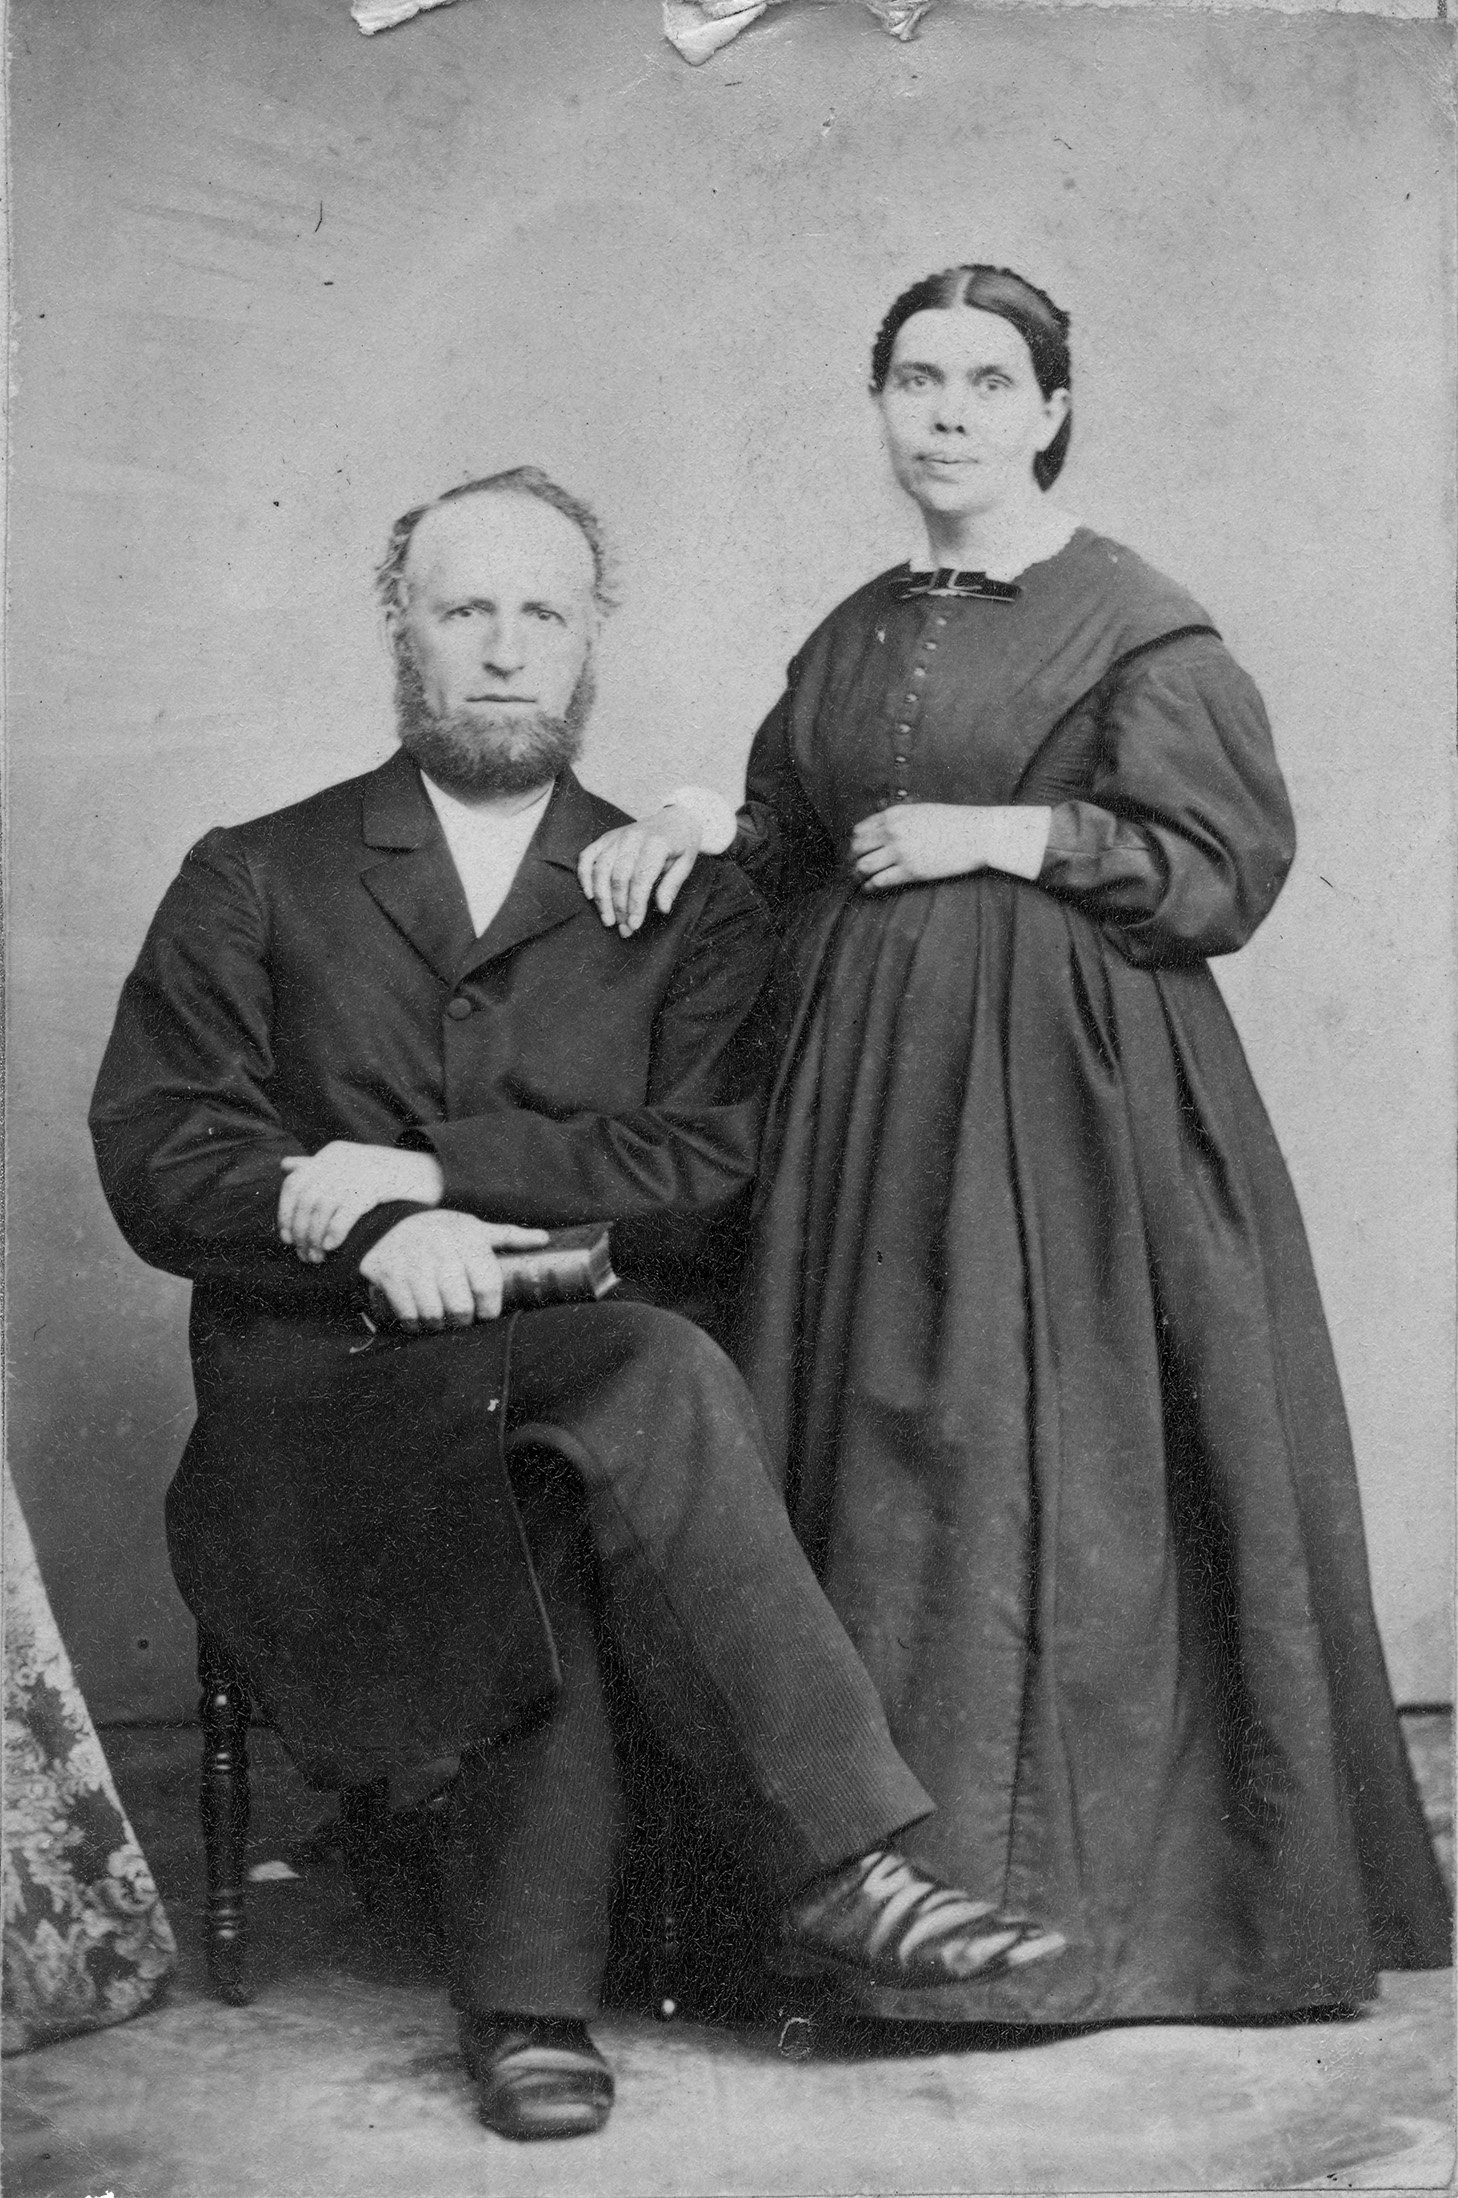
\includegraphics[width=1\linewidth]{images/james-and-ellen-white.jpg}
    \caption*{James Springer White (1821-1881) and Ellen White (1827-1915)}
    \label{fig:james-and-ellen-white}
\end{figure}


\begin{figure}[hp]
    \centering
    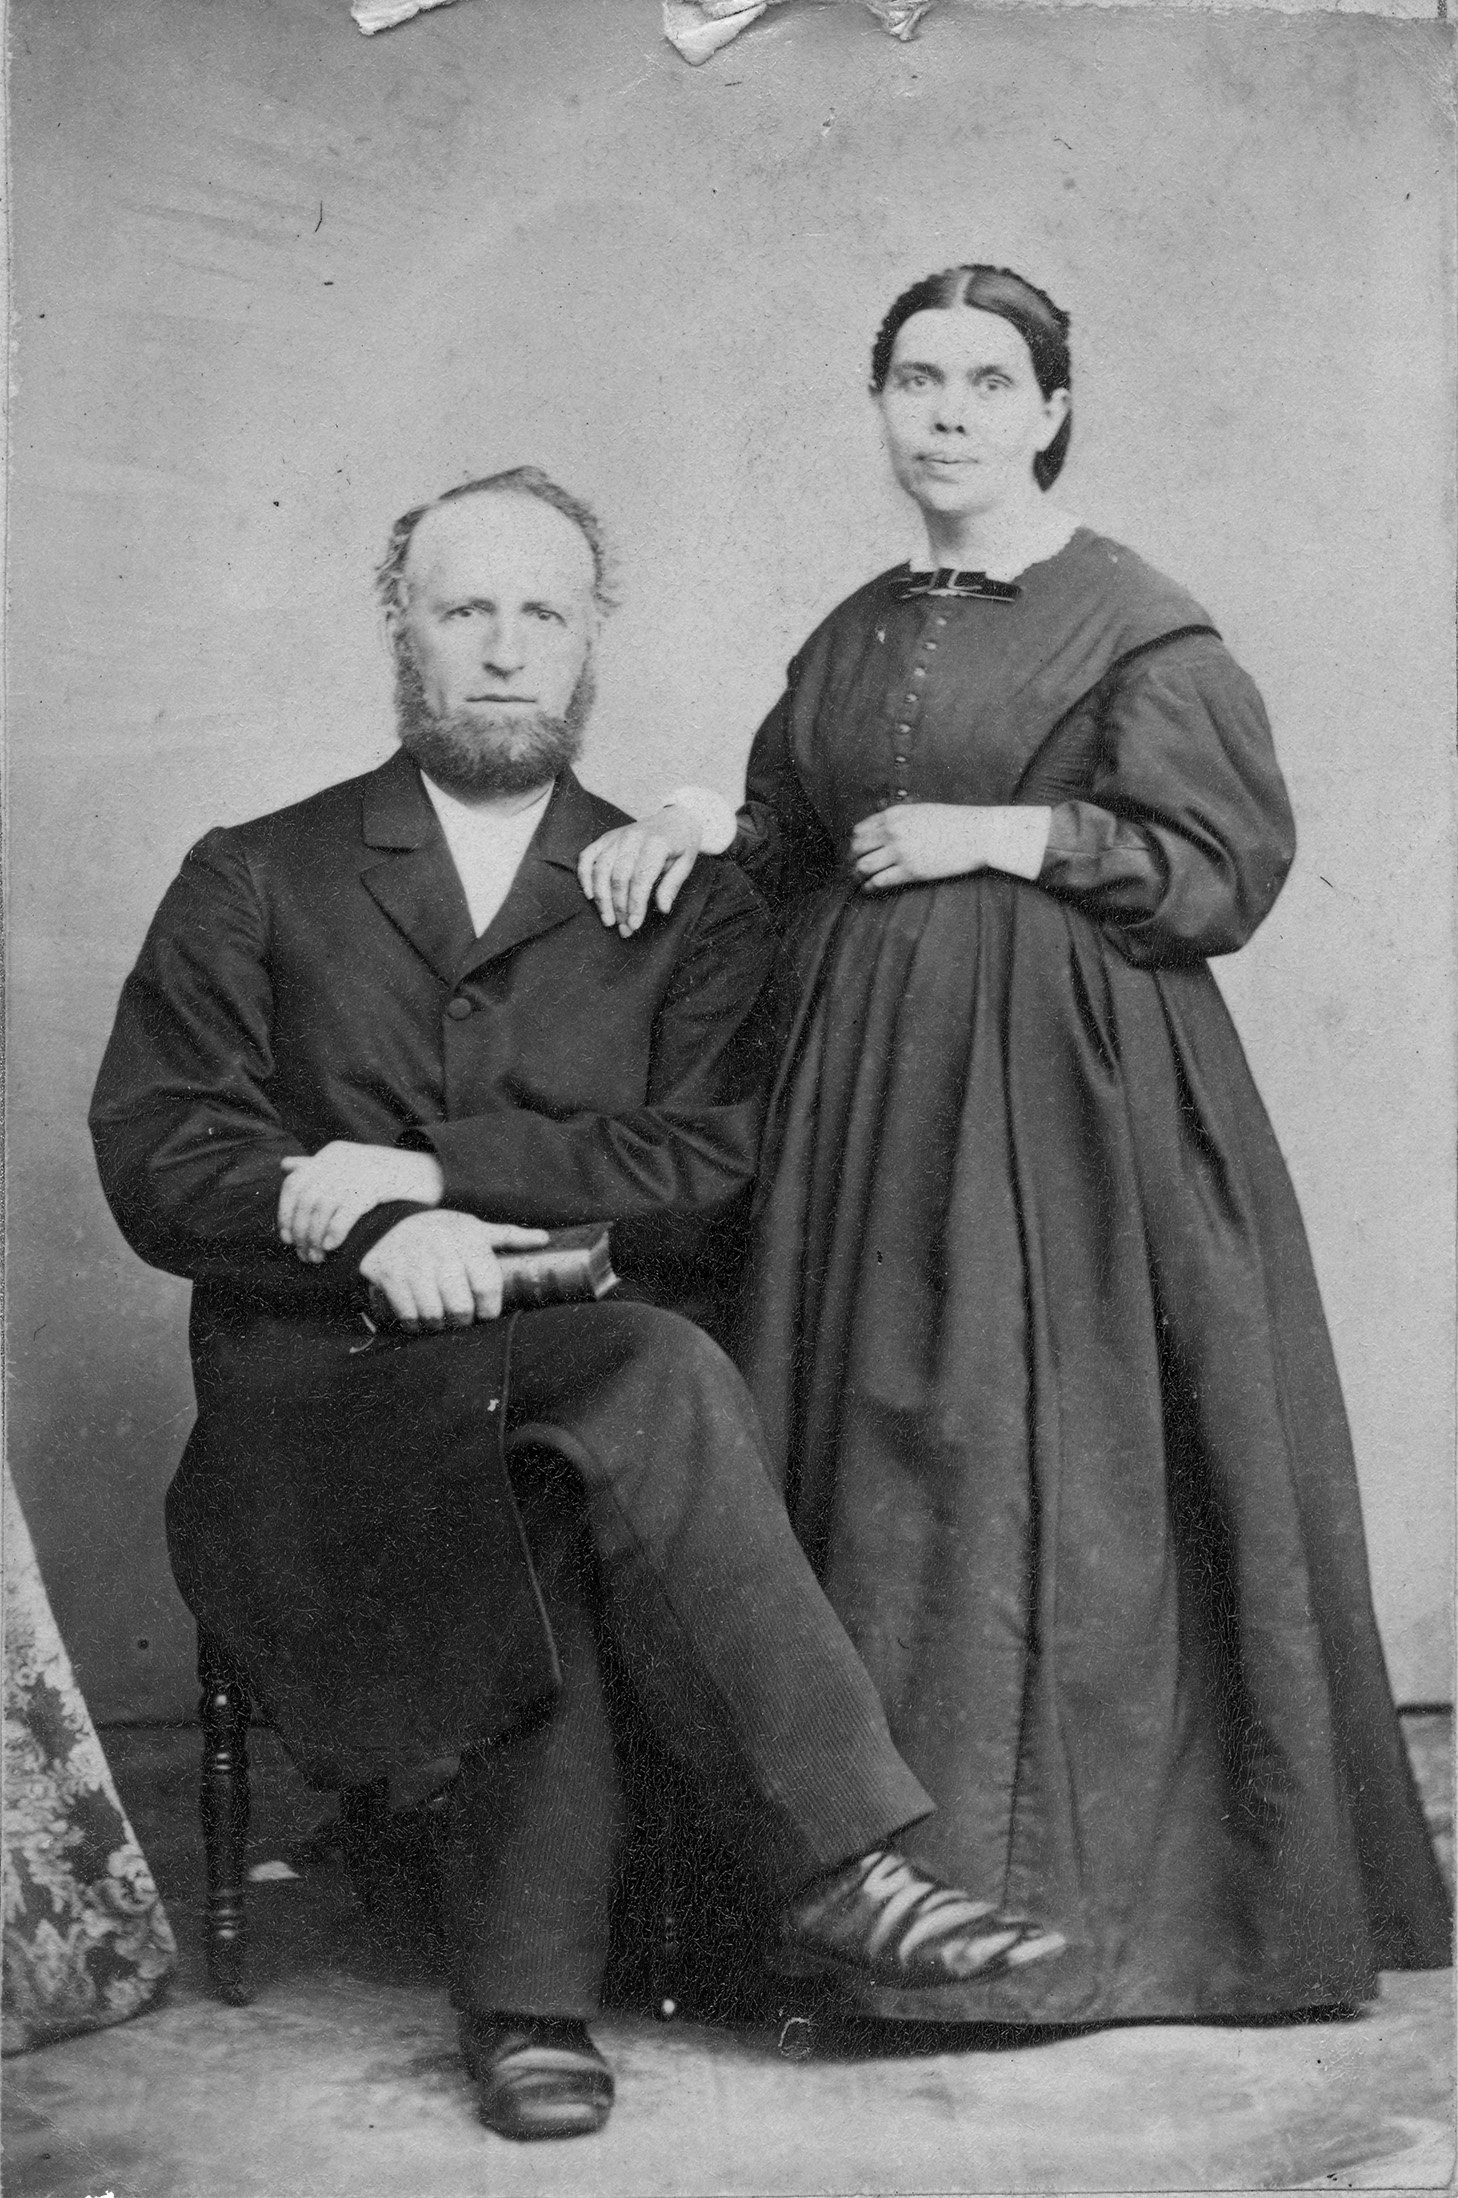
\includegraphics[width=1\linewidth]{images/james-and-ellen-white.jpg}
    \caption*{جيمس سبرينغر وايت (1821-1881) وإلين وايت (1827-1915)}
    \label{fig:james-and-ellen-white}
\end{figure}


\othersQuote{\textbf{MAN was made in the image of God}. ‘And God said, Let us make man in our image, after our likeness.’ ‘So God created man in his own image, in the image of God created he him.’ Genesis 1:26, 27. See also chap. 9:6; 1 Corinthians 11:7. \textbf{Those who deny the personality of God, say that ‘image’ here does not mean \underline{physical form}, but moral image, and they make this the grand starting point to prove the immortality of all men}. The argument stands thus: First, man was made in God’s moral image. Second, God is an immortal being. Third, therefore all men are immortal. But this mode of reasoning would also prove man omnipotent, omniscient, and omnipresent, and thus clothe mortal man with all the attributes of the deity. Let us try it: First, man was made in God’s moral image. Second, God is omnipotent, omniscient, and omnipresent. Third, therefore, man is omnipotent, omniscient, and omnipresent. That which proves too much, proves nothing to the point, therefore the position that the image of God means his moral image, cannot be sustained. \textbf{As proof that God is a person, read his own words to Moses}: ‘And the Lord said, Behold there is a place by me, and thou shalt stand upon a rock; and it shall come to pass, while my glory passeth by, that I will put thee in a cleft of the rock, and will cover thee \textbf{with my hand} while \textbf{I pass by}. And I will take away \textbf{mine hand} and thou shalt \textbf{see my back parts}; \textbf{but my face shall not be seen}.’ Exodus 33:21-23. See also chap. 24:9-11. \textbf{Here God tells Moses that he shall \underline{see his form}}. \textbf{To say that God made it appear to Moses that he saw his form, when he has no form, is charging God with adding to falsehood a sort of juggling deception upon his servant Moses}.}[James S. White, PERGO 1.1; 1861][https://egwwritings.org/read?panels=p1471.3]


\othersQuote{\textbf{خُلِقَ الإنسان على صورة الله}. ‘وقال الله: نعمل الإنسان على صورتنا كشبهنا.’ ‘فخلق الله الإنسان على صورته. على صورة الله خلقه.’ تكوين 1: 26، 27. انظر أيضًا الإصحاح 9: 6؛ 1 كورنثوس 11: 7. \textbf{أولئك الذين ينكرون شخصانية الله، يقولون أن ‘الصورة’ هنا لا تعني \underline{الشكل المادي}، بل الصورة الأخلاقية، ويجعلون هذه نقطة الانطلاق الكبرى لإثبات خلود جميع البشر}. تقوم الحجة على النحو التالي: أولاً، خُلق الإنسان على صورة الله الأخلاقية. ثانيًا، الله كائن خالد. ثالثًا، لذلك جميع البشر خالدون. لكن هذا النمط من التفكير من شأنه أيضًا أن يثبت أن الإنسان كلي القدرة، كلي العلم، وكلي الوجود، وبالتالي يكسو الإنسان الفاني بكل صفات الألوهية. دعونا نجرب ذلك: أولاً، خُلق الإنسان على صورة الله الأخلاقية. ثانيًا، الله كلي القدرة، كلي العلم، وكلي الوجود. ثالثًا، لذلك، الإنسان كلي القدرة، كلي العلم، وكلي الوجود. ما يثبت الكثير جدًا، لا يثبت شيئًا على الإطلاق، لذلك لا يمكن دعم الموقف القائل بأن صورة الله تعني صورته الأخلاقية. \textbf{كدليل على أن الله شخص، اقرأ كلماته الخاصة لموسى}: ‘وقال الرب: هوذا عندي مكان، فتقف على الصخرة، ويكون متى اجتاز مجدي، أني أضعك في نقرة من الصخرة، وأسترك \textbf{بيدي} حتى \textbf{أجتاز}. ثم أرفع \textbf{يدي} فتنظر \textbf{ورائي}، \textbf{وأما وجهي فلا يُرى}.’ خروج 33: 21-23. انظر أيضًا الإصحاح 24: 9-11. \textbf{هنا يخبر الله موسى أنه سيرى \underline{شكله}}. \textbf{القول بأن الله جعل الأمر يبدو لموسى أنه رأى شكله، بينما ليس له شكل، هو اتهام لله بإضافة نوع من الخداع المتلاعب إلى الكذب على خادمه موسى}.}[James S. White, PERGO 1.1; 1861][https://egwwritings.org/read?panels=p1471.3]


\othersQuoteNoGap{But the skeptic thinks he sees a contradiction between verse 11, which says that the Lord spake unto Moses face to face, and verse 20, which states that Moses could not see his face. But let Numbers 12:5-8 remove the difficulty. \textbf{‘And the Lord came down in the pillar of the cloud}, and stood in the door of the tabernacle, and called Aaron and Miriam, and they both came forth. And he said, Hear now my words. If there be a prophet among you, I, the Lord, will make myself known unto him in a vision, and will speak unto him in a dream. My servant Moses is not so, who is faithful in all mine house. \textbf{With him will I speak mouth to mouth, even \underline{apparently}}.’}[James S. White, PERGO 2.1; 1861][https://egwwritings.org/read?panels=p1471.6]


\othersQuoteNoGap{لكن الملحد يعتقد أنه يرى تناقضًا بين الآية 11، التي تقول إن الرب تكلم مع موسى وجهًا لوجه، والآية 20، التي تنص على أن موسى لا يستطيع أن يرى وجهه. لكن دع سفر العدد 12: 5-8 يزيل الصعوبة. \textbf{‘فنزل الرب في عمود السحاب}، ووقف في باب الخيمة، ودعا هارون ومريم، فخرجا كلاهما. فقال: اسمعا كلامي. إن كان منكم نبي للرب، فبالرؤيا أستعلن له. في الحلم أكلمه. وأما عبدي موسى فليس هكذا، بل هو أمين في كل بيتي. \textbf{فمًا إلى فم وعيانًا أتكلم معه، \underline{ظاهرًا}}}.’}[James S. White, PERGO 2.1; 1861][https://egwwritings.org/read?panels=p1471.6]


\othersQuoteNoGap{The great and dreadful God came down, wrapped in a cloud of glory. \textbf{This cloud could be seen, but not the face which possesses more dazzling brightness than a thousand suns}. Under these circumstances Moses was permitted to draw near and \textbf{converse with God face to face, or mouth to mouth, even \underline{apparently}}.}[James S. White, PERGO 2.2; 1861][https://egwwritings.org/read?panels=p1471.7]


\othersQuoteNoGap{نزل الإله العظيم المهيب، ملفوفًا بسحابة من المجد. \textbf{يمكن رؤية هذه السحابة، ولكن ليس الوجه الذي يمتلك سطوعًا أكثر إبهارًا من ألف شمس}. في ظل هذه الظروف، سُمح لموسى بالاقتراب و\textbf{التحدث مع الله وجهًا لوجه، أو فمًا إلى فم، \underline{ظاهرًا}}.}[James S. White, PERGO 2.2; 1861][https://egwwritings.org/read?panels=p1471.7]


\othersQuoteNoGap{Says the prophet Daniel, ‘I beheld till the thrones were cast down, and \textbf{the Ancient of days did sit}, whose garment was white as snow, \textbf{and the hairs of his head like the pure wool}; \textbf{his throne was like the fiery flame, and his wheels as burning fire}.’ Chap. 7:9. ‘I saw in the night visions, and, behold, one like the Son of man came with the clouds of heaven, and \textbf{came to the Ancient of days}, and they brought \textbf{him near before him}, and there was given him dominion and glory and a kingdom.’ Verses 13, 14.}[James S. White, PERGO 2.3; 1861][https://egwwritings.org/read?panels=p1471.8]


\othersQuoteNoGap{يقول النبي دانيال، ‘كنت أرى أنه وضعت عروش، و\textbf{جلس القديم الأيام}. لباسه أبيض كالثلج، \textbf{وشعر رأسه كالصوف النقي}، \textbf{عرشه لهيب نار، وبكراته نار متقدة}.’ الإصحاح 7: 9. ‘كنت أرى في رؤى الليل وإذا مع سحب السماء مثل ابن إنسان \textbf{أتى إلى القديم الأيام}، فقربوه \textbf{قدامه}. فأعطي سلطانًا ومجدًا وملكوتًا.’ الآيات 13، 14.}[James S. White, PERGO 2.3; 1861][https://egwwritings.org/read?panels=p1471.8]


\othersQuoteNoGap{Here is a sublime description of the action of \textbf{two personages}; viz, \textbf{God the Father, and his Son Jesus Christ}. \textbf{Deny their personality, and there is not a distinct idea in these quotations from Daniel}. In connection with this quotation read the apostle’s declaration that \textbf{the Son was in the express image of his Father’s person}. ‘God, who at sundry times, and in divers manners, spake in time past unto the fathers by the prophets, hath in these last days spoken unto us by his Son, whom he hath appointed heir of all things, by whom also he made the worlds; \textbf{who being the brightness of his glory, and the express image of his person}.’ Hebrews 1:1-3.}[James S. White, PERGO 3.1; 1861][https://egwwritings.org/read?panels=p1471.11]


\othersQuoteNoGap{هنا وصف رائع لعمل \textbf{شخصيتين}؛ أي \textbf{الله الآب، وابنه يسوع المسيح}. \textbf{أنكر شخصانيتهما، ولن تجد فكرة واضحة في هذه الاقتباسات من دانيال}. بالاتصال مع هذا الاقتباس اقرأ إعلان الرسول أن \textbf{الابن كان على صورة جوهره}. ‘الله، بعد ما كلم الآباء بالأنبياء قديمًا، بأنواع وطرق كثيرة، كلمنا في هذه الأيام الأخيرة في ابنه، الذي جعله وارثًا لكل شيء، الذي به أيضًا عمل العالمين، \textbf{الذي، وهو بهاء مجده، ورسم جوهره}.’ عبرانيين 1: 1-3.}[James S. White, PERGO 3.1; 1861][https://egwwritings.org/read?panels=p1471.11]


\othersQuoteNoGap{We here add the testimony of Christ. ‘And the Father himself which hath sent me, hath borne witness of me. Ye have neither heard his voice at any time, \textbf{nor seen his shape}.’ John 5:37. See also Philippians 2:6. \textbf{To say that the Father has not a personal shape, seems the most pointed contradiction of plain scripture terms}. \\
OBJECTION. - ‘\textbf{\underline{God is a Spirit}}.’ John 4:24.}[James S. White, PERGO 3.2; 1861][https://egwwritings.org/read?panels=p1471.12]


\othersQuoteNoGap{نضيف هنا شهادة المسيح. ‘والآب نفسه الذي أرسلني يشهد لي. لم تسمعوا صوته قط، \textbf{ولا أبصرتم هيئته}.’ يوحنا 5: 37. انظر أيضًا فيلبي 2: 6. \textbf{القول بأن الآب ليس له هيئة شخصية، يبدو أكثر تناقضًا صريحًا مع عبارات الكتاب المقدس الواضحة}. \\
اعتراض. - ‘\textbf{\underline{الله روح}}.’ يوحنا 4: 24.}[James S. White, PERGO 3.2; 1861][https://egwwritings.org/read?panels=p1471.12]


\othersQuoteNoGap{ANSWER. - \textbf{Angels are also spirits} [Psalm 104:4], yet those that visited Abram and Lot, lay down, ate, and took hold of Lot’s hand. \textbf{They were spirit beings. So is God a Spirit being}.}[James S. White, PERGO 3.3; 1861][https://egwwritings.org/read?panels=p1471.13]


\othersQuoteNoGap{الجواب. - \textbf{الملائكة أيضًا أرواح} [مزمور 104:4]، ومع ذلك فإن أولئك الذين زاروا إبراهيم ولوط، استلقوا، وأكلوا، وأمسكوا بيد لوط. \textbf{كانوا كائنات روحية. وكذلك الله كائن روحي}.}[جيمس س. وايت، PERGO 3.3؛ 1861][https://egwwritings.org/read?panels=p1471.13]


\othersQuoteNoGap{OBJ. - \textbf{God is everywhere}. Proof. Psalm 139:1-8. \textbf{He is as much in every place as in any one place}.}[James S. White, PERGO 3.4; 1861][https://egwwritings.org/read?panels=p1471.14]


\othersQuoteNoGap{اعتراض. - \textbf{الله موجود في كل مكان}. الدليل. مزمور 139:1-8. \textbf{هو موجود في كل مكان بنفس القدر الذي هو موجود فيه في أي مكان واحد}.}[جيمس س. وايت، PERGO 3.4؛ 1861][https://egwwritings.org/read?panels=p1471.14]


\othersQuoteNoGap{ANS. - 1. \textbf{God is everywhere by virtue of his omniscience}, as will be seen by the very words of David referred to above. Verses 1-6. ‘O Lord, \textbf{thou hast searched me, and known me}. \textbf{Thou knowest} my down-sitting and mine uprising; \textbf{thou understandest} my thought afar off. Thou compassest my path and my lying down, and art \textbf{acquainted }with all my ways. For there is not a word in my tongue, but, lo, O Lord, \textbf{thou knowest it altogether}. Thou hast beset me behind and before, and laid thy hand upon me. \textbf{Such knowledge} is too wonderful for me. It is high; I cannot attain unto it.’}[James S. White, PERGO 3.5; 1861][https://egwwritings.org/read?panels=p1471.15]


\othersQuoteNoGap{الجواب. - 1. \textbf{الله موجود في كل مكان بفضل علمه المحيط بكل شيء}، كما سيتضح من كلمات داود نفسها المشار إليها أعلاه. الآيات 1-6. ‘يا رب، \textbf{قد اختبرتني وعرفتني}. \textbf{أنت عرفت} جلوسي وقيامي. \textbf{فهمت} فكري من بعيد. مسلكي ومربضي ذريت، وكل طرقي \textbf{عرفت}. لأنه ليس كلمة في لساني إلا وأنت يا رب \textbf{عرفتها كلها}. من خلف ومن قدام حاصرتني، وجعلت علي يدك. \textbf{هذه المعرفة} عجيبة فوقي. ارتفعت، لا أستطيعها.’}[جيمس س. وايت، PERGO 3.5؛ 1861][https://egwwritings.org/read?panels=p1471.15]


\othersQuoteNoGap{2. \textbf{God is \underline{everywhere by virtue of his Spirit}, \underline{which is his representative}, and is manifested wherever he pleases}, as will be seen by the very words the objector claims, referred to above. Verses 7-10. ‘\textbf{Whither shall I go from \underline{thy Spirit}}? \textbf{or whither shall I flee from \underline{thy presence}}? If I ascend up into heaven, thou art there; if I make my bed in hell, behold, thou art there. If I take the wings of the morning, and dwell in the uttermost parts of the sea, even there shall thy hand lead me, and thy right hand shall hold me.’}[James S. White, PERGO 4.1; 1861][https://egwwritings.org/read?panels=p1471.18]


\othersQuoteNoGap{2. \textbf{الله \underline{موجود في كل مكان بفضل روحه}، \underline{التي هي ممثله}، وتظهر حيثما يشاء}، كما سيتضح من الكلمات نفسها التي يستشهد بها المعترض، المشار إليها أعلاه. الآيات 7-10. ‘\textbf{أين أذهب من \underline{روحك}}؟ \textbf{ومن \underline{حضرتك} أين أهرب}؟ إن صعدت إلى السماوات فأنت هناك، وإن فرشت في الهاوية فها أنت. إن أخذت جناحي الصبح، وسكنت في أقاصي البحر، فهناك أيضًا تهديني يدك وتمسكني يمينك.’}[جيمس س. وايت، PERGO 4.1؛ 1861][https://egwwritings.org/read?panels=p1471.18]


\othersQuoteNoGap{\textbf{God is in heaven.} This we are taught in the Lord’s prayer. ‘\textbf{Our Father which art in heaven}.’ Matthew 6:9; Luke 11:2. \textbf{But if God is as much in every place as he is in any one place, then heaven is also as much in every place as it is in any one place, and the idea of going to heaven is all a mistake}. We are all in heaven; and the Lord’s prayer, according to this foggy theology simply means, Our Father \textbf{which art everywhere,} hallowed be thy name. Thy kingdom come, thy will be done, on earth, \textbf{as it is everywhere}.}[James S. White, PERGO 4.2; 1861][https://egwwritings.org/read?panels=p1471.19]


\othersQuoteNoGap{\textbf{الله في السماء.} هذا ما تعلمنا إياه صلاة الرب. ‘\textbf{أبانا الذي في السماوات}.’ متى 6:9؛ لوقا 11:2. \textbf{ولكن إذا كان الله موجودًا في كل مكان بنفس القدر الذي هو موجود فيه في أي مكان واحد، فإن السماء أيضًا موجودة في كل مكان بنفس القدر الذي هي موجودة فيه في أي مكان واحد، وفكرة الذهاب إلى السماء كلها خطأ}. نحن جميعًا في السماء؛ وصلاة الرب، وفقًا لهذا اللاهوت الضبابي، تعني ببساطة، أبانا \textbf{الذي في كل مكان،} ليتقدس اسمك. ليأت ملكوتك، لتكن مشيئتك، على الأرض، \textbf{كما هي في كل مكان}.}[جيمس س. وايت، PERGO 4.2؛ 1861][https://egwwritings.org/read?panels=p1471.19]


\othersQuoteNoGap{Again, Bible readers have believed that Enoch and Elijah were really taken up \textbf{to God in heaven}. \textbf{But if God and heaven be as much in every place as in any one place, this is all a mistake}. They were not translated. And all that is said about the chariot of fire, and horses of fire, and the attending whirlwind to take Elijah up into heaven, was a useless parade. They only evaporated, and a misty vapor passed through the entire universe. This is all of Enoch and Elijah that the mind can possibly grasp, \textbf{admitting that God and heaven are no more in any one place than in every place}. But it is said of Elijah that he ‘\textbf{went up} by a whirlwind \textbf{into heaven}.’ 2 Kings 2:11. And of Enoch it is said that he ‘walked with God, and was not, for God took him.’ Genesis 5:24.}[James S. White, PERGO 4.3; 1861][https://egwwritings.org/read?panels=p1471.20]


\othersQuoteNoGap{مرة أخرى، آمن قراء الكتاب المقدس أن أخنوخ وإيليا قد أُخذا حقًا \textbf{إلى الله في السماء}. \textbf{ولكن إذا كان الله والسماء موجودين في كل مكان بنفس القدر الذي هما موجودان فيه في أي مكان واحد، فهذا كله خطأ}. لم يتم نقلهما. وكل ما قيل عن مركبة النار، وخيول النار، والزوبعة المرافقة لأخذ إيليا إلى السماء، كان استعراضًا غير ضروري. لقد تبخرا فقط، وانتشر بخار ضبابي عبر الكون بأكمله. هذا كل ما يمكن للعقل أن يفهمه عن أخنوخ وإيليا، \textbf{إذا سلمنا بأن الله والسماء ليسا في أي مكان واحد أكثر مما هما في كل مكان}. ولكن قيل عن إيليا أنه ‘\textbf{صعد} في العاصفة \textbf{إلى السماء}.’ 2 ملوك 2:11. وقيل عن أخنوخ أنه ‘سار مع الله، ولم يوجد لأن الله أخذه.’ تكوين 5:24.}[جيمس س. وايت، PERGO 4.3؛ 1861][https://egwwritings.org/read?panels=p1471.20]


\othersQuoteNoGap{\textbf{Jesus is said to be on the right hand of the Majesty on high}. Hebrews 1:3. ‘So, then, after the Lord had spoken unto them \textbf{he was received \underline{up into heaven}}, \textbf{and sat on the right hand of God}.’ Mark 16:19. \textbf{But if heaven be everywhere, and God everywhere, then Christ’s ascension up to heaven, at the Father’s right hand, simply means that he went everywhere}! He was only taken up where the cloud hid him from the gaze of his disciples, and then evaporated and went everywhere! So that instead of the lovely Jesus, so beautifully described in both Testaments, we have only a sort of essence dispersed through the entire universe. And in harmony with this rarified theology, Christ’s second advent, or his return, would be the condensation of this essence to some locality, say the mount of Olivet! \textbf{Christ arose from the dead with a physical form}. ‘He is not here,’ said the angel, ‘for he is risen as he said.’ Matthew 28:6.}[James S. White, PERGO 5.1; 1861][https://egwwritings.org/read?panels=p1471.23]


\othersQuoteNoGap{\textbf{يقال إن يسوع عن يمين العظمة في الأعالي}. عبرانيين 1:3. ‘ثم إن الرب بعدما كلمهم \textbf{ارتفع \underline{إلى السماء}}، \textbf{وجلس عن يمين الله}.’ مرقس 16:19. \textbf{ولكن إذا كانت السماء في كل مكان، والله في كل مكان، فإن صعود المسيح إلى السماء، عن يمين الآب، يعني ببساطة أنه ذهب إلى كل مكان}! لقد أُخذ فقط حيث أخفته السحابة عن أنظار تلاميذه، ثم تبخر وذهب إلى كل مكان! بحيث أنه بدلاً من يسوع المحبوب، الموصوف بشكل جميل في كلا العهدين، لدينا فقط نوع من الجوهر منتشر في جميع أنحاء الكون. وانسجامًا مع هذا اللاهوت المخفف، فإن مجيء المسيح الثاني، أو عودته، ستكون تكثيفًا لهذا الجوهر في مكان ما، لنقل جبل الزيتون! \textbf{قام المسيح من الأموات بشكل جسدي}. ‘ليس هو ههنا،‘ قال الملاك، ‘لأنه قام كما قال.’ متى 28:6.}[جيمس س. وايت، PERGO 5.1؛ 1861][https://egwwritings.org/read?panels=p1471.23]


\othersQuoteNoGap{‘And as they went to tell his disciples, behold, Jesus met them, saying, All hail! And they came and \textbf{held him by the feet}, and they worshiped him.’ Verse 9.}[James S. White, PERGO 5.2; 1861][https://egwwritings.org/read?panels=p1471.24]


\othersQuoteNoGap{‘وفيما هما منطلقتان لتخبرا تلاميذه إذا يسوع لاقاهما وقال: سلام لكما. فتقدمتا \textbf{وأمسكتا بقدميه}، وسجدتا له.’ الآية 9.}[جيمس س. وايت، PERGO 5.2؛ 1861][https://egwwritings.org/read?panels=p1471.24]


\othersQuoteNoGap{‘\textbf{Behold my hands and my feet},’ said Jesus to those who stood in doubt of his resurrection, ‘that it is I myself. \textbf{Handle me and see, \underline{for a spirit hath not flesh and bones} as ye see me have}. And when he had thus spoken, he \textbf{showed them his hands and his feet}. And while they yet believed not for joy, and wondered, he said unto them, Have ye here any meat? And they gave him a piece of broiled fish, and of an honey-comb, and he took it and did eat before them.’ Luke 24:39-43.}[James S. White, PERGO 5.3; 1861][https://egwwritings.org/read?panels=p1471.25]


\othersQuoteNoGap{‘\textbf{انظروا يدي ورجلي}،‘ قال يسوع لأولئك الذين كانوا في شك من قيامته، ‘إني أنا هو. \textbf{جسوني وانظروا، \underline{فإن الروح ليس له لحم وعظام} كما ترون لي}. وحين قال هذا \textbf{أراهم يديه ورجليه}. وبينما هم غير مصدقين من الفرح، ومتعجبون، قال لهم: أعندكم ههنا طعام؟ فناولوه جزءًا من سمك مشوي، وشيئًا من شهد عسل. فأخذ وأكل قدامهم.’ لوقا 24:39-43.}[جيمس س. وايت، PERGO 5.3؛ 1861][https://egwwritings.org/read?panels=p1471.25]


\othersQuoteNoGap{After Jesus addressed his disciples on the mount of Olivet, he \textbf{was taken up from them}, and a cloud received him out of their sight. ‘And while they looked steadfastly \textbf{toward heaven as he went up,} behold two men stood by them in white apparel, which also said, Ye men of Galilee, why stand ye gazing up into heaven? This same Jesus which is \textbf{taken up from you into heaven}, shall so come in like manner as ye have seen him \textbf{go into heaven}.’ Acts 1:9-11. J. W.}[James S. White, PERGO 6.1; 1861][https://egwwritings.org/read?panels=p1471.27]


\othersQuoteNoGap{بعد أن خاطب يسوع تلاميذه على جبل الزيتون، \textbf{ارتفع عنهم}، وأخذته سحابة عن أعينهم. ‘وفيما كانوا يشخصون \textbf{إلى السماء وهو منطلق}، إذا رجلان قد وقفا بهم بلباس أبيض، وقالا: أيها الرجال الجليليون، ما بالكم واقفين تنظرون إلى السماء؟ إن يسوع هذا الذي \textbf{ارتفع عنكم إلى السماء}، سيأتي هكذا كما رأيتموه \textbf{منطلقًا إلى السماء}.’ أعمال 1:9-11. ج. و.}[جيمس س. وايت، PERGO 6.1؛ 1861][https://egwwritings.org/read?panels=p1471.27]


James White fights the idea that God is just a spirit, and as such, is present \others{as much in every place as in any one place}. He gives plain and positive testimony from Scripture that God is a personal being; we see the very same sentiments in Ellen White’s writings.


يحارب جيمس وايت فكرة أن الله هو مجرد روح، وبالتالي، موجود \others{في كل مكان بنفس القدر كما في أي مكان واحد}. يقدم شهادة واضحة وإيجابية من الكتاب المقدس أن الله كائن شخصي؛ نرى نفس الآراء في كتابات إلين وايت.


\egw{The mighty power that works through all nature and sustains all things is not, as some men of science claim, \textbf{merely an all-pervading principle}, an actuating energy. \textbf{\underline{God is a spirit; yet He is a personal being}}, \textbf{for man was made in His image}. \textbf{As \underline{a personal being}}, God has revealed Himself in His Son. Jesus, the outshining of the Father’s glory, “and \textbf{the express \underline{image of His person}}” (Hebrews 1:3), was on earth found in fashion as a man. As \textbf{a personal Saviour} He came to the world. As \textbf{a personal Saviour He ascended \underline{on high}}. As \textbf{a personal Saviour He intercedes \underline{in the heavenly courts}}. \textbf{Before the throne of God} in our behalf ministers “One like the Son of man.” Daniel 7:13.}[Ed 131.5; 1903][https://egwwritings.org/read?panels=p29.632]


\egw{إن القوة العظيمة التي تعمل في كل الطبيعة وتعضد كل الأشياء ليست، كما يدعي بعض رجال العلم، \textbf{مجرد مبدأ منتشر في كل مكان}، طاقة محركة. \textbf{\underline{الله روح؛ ومع ذلك فهو كائن شخصي}}، \textbf{لأن الإنسان خُلق على صورته}. \textbf{بصفته \underline{كائنًا شخصيًا}}، أعلن الله عن نفسه في ابنه. يسوع، إشراق مجد الآب، “و\textbf{\underline{صورة جوهره}}” (عبرانيين ١:٣)، وُجد على الأرض في هيئة إنسان. \textbf{كمخلص شخصي} جاء إلى العالم. \textbf{كمخلص شخصي صعد \underline{إلى العلاء}}. \textbf{كمخلص شخصي يشفع \underline{في المحاكم السماوية}}. \textbf{أمام عرش الله} يخدم نيابة عنا “شبه ابن إنسان.” دانيال ٧:١٣.}[Ed 131.5; 1903][https://egwwritings.org/read?panels=p29.632]


Ellen White and the Adventist pioneers made a distinction between the terms ‘\textit{spirit}’ and ‘\textit{being}’. God is a personal being, not just a spirit. He is not\others{as much in every place as in any one place}, but He is\others{in one place more than another}[John. N. Loughborough, “Is God a Person?” The Adventist Review and Sabbath Herald, September 18, 1855][https://documents.adventistarchives.org/Periodicals/RH/RH18550918-V07-06.pdf]. He is in heaven, in His temple, sitting on His throne—in person—and He is everywhere present by His representative, the Holy Spirit.


ميزت إلين وايت ورواد الأدفنتست بين مصطلحي ‘\textit{روح}’ و’\textit{كائن}’. الله كائن شخصي، وليس مجرد روح. هو ليس \others{في كل مكان بنفس القدر كما في أي مكان واحد}، بل هو \others{في مكان واحد أكثر من آخر}[John. N. Loughborough, “Is God a Person?” The Adventist Review and Sabbath Herald, September 18, 1855][https://documents.adventistarchives.org/Periodicals/RH/RH18550918-V07-06.pdf]. إنه في السماء، في هيكله، جالسًا على عرشه—بشخصه—وهو موجود في كل مكان بواسطة ممثله، الروح القدس.


Here are some other quotations from Sister White that are in harmony with the pioneers’ views on the \emcap{personality of God}:


فيما يلي بعض الاقتباسات الأخرى من الأخت وايت التي تتوافق مع آراء الرواد حول \emcap{شخصانية الله}:


\egw{He \normaltext{[Jesus]} taught that God was a rewarder of the righteous, and a punisher of the transgressor. \textbf{He was not an intangible spirit}, but a living ruler of the universe. \textbf{This gracious Father} was constantly working for the good of man, and mindful of all that concerns him...}[3SP 47.1; 1878][https://egwwritings.org/read?panels=p142.195]


\egw{لقد علّم \normaltext{[يسوع]} أن الله يكافئ الأبرار، ويعاقب المتعدي. \textbf{لم يكن روحًا غير ملموسة}، بل حاكمًا حيًا للكون. \textbf{هذا الأب الرحيم} كان يعمل باستمرار من أجل خير الإنسان، ومهتمًا بكل ما يخصه...}[3SP 47.1; 1878][https://egwwritings.org/read?panels=p142.195]


\egw{\textbf{The Bible shows us \underline{God in His high and holy place}}, not in a state of inactivity, not in silence and solitude, but surrounded by ten thousand times ten thousand and thousands of thousands of holy beings, all waiting to do His will. \textbf{Through these messengers He is in active communication with every part of His dominion}. \textbf{\underline{By His Spirit He is everywhere present}}. \textbf{Through the agency of His Spirit and His angels} He ministers to the children of men.}[MH 417.2; 1905][https://egwwritings.org/read?panels=p135.2136]


\egw{\textbf{يُظهر لنا الكتاب المقدس \underline{الله في مكانه العالي والمقدس}}، ليس في حالة من الخمول، وليس في صمت وعزلة، بل محاطًا بعشرة آلاف مرة عشرة آلاف وألوف ألوف من الكائنات المقدسة، كلها تنتظر لتنفيذ مشيئته. \textbf{من خلال هؤلاء الرسل هو في اتصال نشط مع كل جزء من ملكوته}. \textbf{\underline{بروحه هو موجود في كل مكان}}. \textbf{من خلال وكالة روحه وملائكته} يخدم أبناء البشر.}[MH 417.2; 1905][https://egwwritings.org/read?panels=p135.2136]


\egw{The greatness of God is to us incomprehensible. ‘\textbf{The Lord’s throne is in heaven}’ (Psalm 11:4); \textbf{\underline{yet by His Spirit He is everywhere present}}. \textbf{He has an intimate knowledge} of, and a personal interest in, all the works of His hand.}[Ed 132.2; 1903][https://egwwritings.org/read?panels=p29.636]


\egw{عظمة الله بالنسبة لنا غير قابلة للإدراك. ‘\textbf{عرش الرب في السماء}’ (مزمور ١١:٤)؛ \textbf{\underline{ومع ذلك فهو بروحه موجود في كل مكان}}. \textbf{لديه معرفة وثيقة} بكل أعمال يديه، واهتمام شخصي بها.}[Ed 132.2; 1903][https://egwwritings.org/read?panels=p29.636]


\egw{Through Jesus Christ, \textbf{God—not a perfume, \underline{not something intangible}, \underline{but a personal God}}—created man and endowed him with intelligence and power.}[Ms117-1898.10; 1898][https://egwwritings.org/read?panels=p7182.15]


\egw{من خلال يسوع المسيح، \textbf{الله—ليس عطرًا، \underline{ليس شيئًا غير ملموس}، \underline{بل إله شخصي}}—خلق الإنسان وزوده بالذكاء والقوة.}[Ms117-1898.10; 1898][https://egwwritings.org/read?panels=p7182.15]


Continuing in James White’s pamphlet, we read his sharp criticism on the notion of an immaterial God. Before that, let’s briefly recall Dr. Kellogg’s argument that\others{\textbf{\underline{Discussions respecting the form of God are utterly unprofitable}}}[Dr. John H. Kellogg, The Living Temple, p.33.][https://archive.org/details/J.H.Kellogg.TheLivingTemple1903/page/n33/] because God is\others{\textbf{far beyond our comprehension }\textbf{\underline{as are the bounds of space and time}}}. He believed that God’s person is not constrained to one locality because He is in\others{as much in every place as in any one place}[James S. White, PERGO 4.3; 1861][https://egwwritings.org/read?panels=p1471.20] \footnote{In the Living Temple, Dr. Kellogg objected that God cannot be everywhere presente at once: “\textit{Says one}, ‘God may be present by his Spirit, or by his power, but certainly God himself \textit{cannot be present everywhere at once}.’ We answer: How can power be separated from the source of power? Where God’s Spirit is at work, where God’s power is manifested, God \textit{himself is actually and truly present}…” \href{https://archive.org/details/J.H.Kellogg.TheLivingTemple1903/page/n29/}{John H. Kellogg, The Living Temple, p.28}.}. If God in His personality were truly a definite being, having a tangible body, then He would not be able to be present\others{as much in every place as in any one place} and, thus, sustain life. James White continues against the reasoning that God is immaterial in His person.


استمرارًا في كتيب جيمس وايت، نقرأ نقده الحاد لفكرة الله غير المادي. قبل ذلك، دعونا نتذكر بإيجاز حجة الدكتور كيلوغ بأن \others{\textbf{\underline{المناقشات المتعلقة بشكل الله عديمة الفائدة تمامًا}}}[Dr. John H. Kellogg, The Living Temple, p.33.][https://archive.org/details/J.H.Kellogg.TheLivingTemple1903/page/n33/] لأن الله \others{\textbf{يتجاوز فهمنا بكثير }\textbf{\underline{كما هي حدود الزمان والمكان}}}. كان يعتقد أن شخص الله لا يقتصر على مكان واحد لأنه موجود \others{في كل مكان بنفس القدر كما في أي مكان واحد}[James S. White, PERGO 4.3; 1861][https://egwwritings.org/read?panels=p1471.20] \footnote{في كتاب ذا ليفينغ تمبل، اعترض الدكتور كيلوغ على أن الله لا يمكن أن يكون موجودًا في كل مكان في وقت واحد: “\textit{يقول أحدهم}، ‘قد يكون الله موجودًا بروحه، أو بقوته، ولكن بالتأكيد الله نفسه \textit{لا يمكن أن يكون موجودًا في كل مكان في وقت واحد}.’ نجيب: كيف يمكن فصل القوة عن مصدر القوة؟ حيث يعمل روح الله، حيث تتجلى قوة الله، الله \textit{نفسه موجود فعليًا وحقًا}...” \href{https://archive.org/details/J.H.Kellogg.TheLivingTemple1903/page/n29/}{John H. Kellogg, The Living Temple, p.28}.}. إذا كان الله في شخصانيته كائنًا محددًا حقًا، له جسد ملموس، فلن يكون قادرًا على أن يكون موجودًا \others{في كل مكان بنفس القدر كما في أي مكان واحد} وبالتالي، يحافظ على الحياة. يواصل جيمس وايت ضد المنطق القائل بأن الله غير مادي في شخصه.


\othersQuote{IMMATERIALITY}


\othersQuote{اللامادية}


\othersQuoteNoGap{\textbf{THIS is but another name for nonentity}. \textbf{It is the negative of all} \textbf{things and} \textbf{\underline{beings} }- of all existence. There is not one particle of proof to be advanced to establish its existence. It has no way to manifest itself to any intelligence in heaven or on earth. \textbf{Neither God, angels, nor men could possibly conceive of such a substance, being, or thing}. \textbf{It possesses no property or power by which \underline{to make itself manifest to any intelligent being} in the universe}. Reason and analogy never scan it, or even conceive of it. \textbf{Revelation never reveals it, nor do any of our senses witness its existence}. \textbf{It cannot be seen, felt, heard, tasted, or smelled, even by the strongest organs, or the most acute sensibilities}. It is neither liquid nor solid, soft nor hard - it can neither extend nor contract. In short, it can exert no influence whatever - it can neither act nor be acted upon. And even if it does exist, it can be of no possible use. It possesses no one, desirable property, faculty, or use, yet, strange to say, \textbf{immateriality is the modern Christian’s God}, \textbf{his anticipated heaven}, \textbf{his immortal self} - \textbf{his all}!}[James S. White, PERGO 6.2; 1861][https://egwwritings.org/read?panels=p1471.29]


\othersQuoteNoGap{\textbf{هذا ليس سوى اسم آخر للعدم}. \textbf{إنه نفي لكل} \textbf{الأشياء و} \textbf{\underline{الكائنات} }- لكل وجود. لا توجد ذرة واحدة من الدليل يمكن تقديمها لإثبات وجودها. ليس لديها وسيلة لإظهار نفسها لأي ذكاء في السماء أو على الأرض. \textbf{لا يمكن لله ولا للملائكة ولا للبشر أن يتصوروا مثل هذه المادة أو الكائن أو الشيء}. \textbf{لا تمتلك أي خاصية أو قوة \underline{لتجعل نفسها ظاهرة لأي كائن ذكي} في الكون}. العقل والقياس لا يستطيعان فحصها، أو حتى تصورها. \textbf{الوحي لا يكشفها أبدًا، ولا تشهد أي من حواسنا على وجودها}. \textbf{لا يمكن رؤيتها أو الشعور بها أو سماعها أو تذوقها أو شمها، حتى بأقوى الأعضاء، أو أكثر الحساسيات حدة}. إنها ليست سائلة ولا صلبة، ناعمة ولا صلبة - لا يمكنها التمدد ولا الانكماش. باختصار، لا يمكنها ممارسة أي تأثير على الإطلاق - لا يمكنها أن تفعل ولا أن يُفعل بها. وحتى لو كانت موجودة، فلا يمكن أن تكون ذات فائدة ممكنة. لا تمتلك أي خاصية أو قدرة أو استخدام مرغوب فيه، ومع ذلك، من الغريب أن نقول، \textbf{اللامادية هي إله المسيحي الحديث}، \textbf{سماؤه المتوقعة}، \textbf{ذاته الخالدة} - \textbf{كل شيء له}!}[James S. White, PERGO 6.2; 1861][https://egwwritings.org/read?panels=p1471.29]


\othersQuoteNoGap{\textbf{O sectarianism! O atheism!! O annihilation!!!} \textbf{who can perceive the nice shades of difference between the one and the other?} They seem alike, all but in name. \textbf{The atheist has no God. \underline{The sectarian has a God without body or parts}.} Who can define the difference? For our part we do not perceive a difference of a single hair; \textbf{they both claim to be the negative of all things which exist} - and both are equally powerless and unknown.}[James S. White, PERGO 6.3; 1861][https://egwwritings.org/read?panels=p1471.30]


\othersQuoteNoGap{\textbf{يا للطائفية! يا للإلحاد!! يا للفناء!!!} \textbf{من يستطيع إدراك الفروق الدقيقة بين الواحد والآخر؟} يبدون متشابهين، إلا في الاسم. \textbf{الملحد ليس لديه إله. \underline{الطائفي لديه إله بدون جسد أو أجزاء}.} من يستطيع تحديد الفرق؟ من جانبنا لا نرى فرقًا بمقدار شعرة واحدة؛ \textbf{كلاهما يدعي أنه نفي لكل الأشياء الموجودة} - وكلاهما عاجز ومجهول بنفس القدر.}[James S. White, PERGO 6.3; 1861][https://egwwritings.org/read?panels=p1471.30]


\othersQuoteNoGap{\textbf{The atheist has no after life, or conscious existence beyond the grave. The sectarian has one, \underline{but it is immaterial, like his God; and without body or parts}. Here again both are negative, and both arrive at the same point}. Their faith and hope amount to the same; only it is expressed by different terms.}[James S. White, PERGO 7.1; 1861][https://egwwritings.org/read?panels=p1471.33]


\othersQuoteNoGap{\textbf{الملحد ليس لديه حياة أخرى، أو وجود واعٍ بعد القبر. الطائفي لديه واحدة، \underline{لكنها غير مادية، مثل إلهه؛ وبدون جسد أو أجزاء}. هنا مرة أخرى كلاهما سلبي، وكلاهما يصل إلى نفس النقطة}. إيمانهما وأملهما يصلان إلى نفس الشيء؛ فقط يتم التعبير عنهما بمصطلحات مختلفة.}[James S. White, PERGO 7.1; 1861][https://egwwritings.org/read?panels=p1471.33]


\othersQuoteNoGap{Again, \textbf{the atheist has no heaven in eternity}. \textbf{The sectarian has one, but it is \underline{immaterial in all its properties}, and is therefore the negative of all riches and substances}. Here again they are equal, and arrive at the same point.}[James S. White, PERGO 7.2; 1861][https://egwwritings.org/read?panels=p1471.34]


\othersQuoteNoGap{مرة أخرى، \textbf{الملحد ليس لديه سماء في الأبدية}. \textbf{الطائفي لديه واحدة، لكنها \underline{غير مادية في كل خصائصها}، وبالتالي فهي نفي لكل الثروات والمواد}. هنا مرة أخرى هما متساويان، ويصلان إلى نفس النقطة.}[James S. White, PERGO 7.2; 1861][https://egwwritings.org/read?panels=p1471.34]


\othersQuoteNoGap{As we do not envy them the possession of all they claim, we will now leave them in the quiet and undisturbed enjoyment of the same, and proceed to examine the portion still left for the despised materialist to enjoy.}[James S. White, PERGO 7.3; 1861][https://egwwritings.org/read?panels=p1471.35]


\othersQuoteNoGap{بما أننا لا نحسدهم على امتلاك كل ما يدعونه، سنتركهم الآن في التمتع الهادئ وغير المزعج بذلك، ونمضي لفحص الجزء المتبقي للماديين المحتقرين للاستمتاع به.}[James S. White, PERGO 7.3; 1861][https://egwwritings.org/read?panels=p1471.35]


\othersQuoteNoGap{\textbf{What is God? He is material, organized intelligence, \underline{possessing both body and parts}. Man is in his image.}}[James S. White, PERGO 7.4; 1861][https://egwwritings.org/read?panels=p1471.36]


\othersQuoteNoGap{\textbf{ما هو الله؟ هو ذكاء مادي منظم، \underline{يمتلك جسدًا وأجزاءً}. الإنسان على صورته.}}[James S. White, PERGO 7.4; 1861][https://egwwritings.org/read?panels=p1471.36]


\othersQuoteNoGap{\textbf{What is Jesus Christ? He is the Son of God, and is \underline{like his Father}, being ‘the brightness of his Father’s glory, and the express image of his person.’ \underline{He is a material intelligence, with body, parts}, and passions; possessing immortal flesh and immortal bones}.}[James S. White, PERGO 7.5; 1861][https://egwwritings.org/read?panels=p1471.37]


\othersQuoteNoGap{\textbf{ما هو يسوع المسيح؟ هو ابن الله، وهو \underline{مثل أبيه}، كونه ‘ضياء مجد أبيه، وصورة جوهره’. \underline{إنه ذكاء مادي، بجسد وأجزاء} وعواطف؛ يمتلك لحمًا خالدًا وعظامًا خالدة}.}[James S. White, PERGO 7.5; 1861][https://egwwritings.org/read?panels=p1471.37]


\othersQuoteNoGap{\textbf{What are men?} They are the offspring of Adam. \textbf{They are capable of receiving intelligence and exaltation to such a degree as to be \underline{raised from the dead with a body like that of Jesus Christ}, \underline{and to possess immortal flesh and bones}}. Thus perfected, they will possess \textbf{the material universe}, that is, the earth, as their ‘everlasting inheritance.’ With these hopes and prospects before us, we say to the Christian world who hold to immateriality, that they are welcome to their God - their life - their heaven, and their all. They claim nothing but that which we throw away; and we claim nothing but that which they throw away. \textbf{Therefore, there is no ground for quarrel or contention between us}.}[James S. White, PERGO 7.6; 1861][https://egwwritings.org/read?panels=p1471.38]


\othersQuoteNoGap{\textbf{ما هم البشر؟} هم نسل آدم. \textbf{هم قادرون على تلقي الذكاء والارتقاء إلى درجة \underline{يُقامون فيها من الموت بجسد مثل جسد يسوع المسيح}، \underline{وامتلاك لحم وعظام خالدة}}. وهكذا بعد اكتمالهم، سيمتلكون \textbf{الكون المادي}، أي الأرض، كـ “ميراثهم الأبدي”. مع هذه الآمال والتوقعات أمامنا، نقول للعالم المسيحي الذي يتمسك باللامادية، أنهم مرحب بهم بإلههم - حياتهم - سمائهم، وكل شيء لهم. هم لا يطالبون بشيء سوى ما نرميه نحن بعيدًا؛ ونحن لا نطالب بشيء سوى ما يرمونه هم بعيدًا. \textbf{لذلك، لا يوجد أساس للخلاف أو النزاع بيننا}.}[James S. White, PERGO 7.6; 1861][https://egwwritings.org/read?panels=p1471.38]


\othersQuoteNoGap{We choose all substance - what remains \\
The mystical sectarian gains; \\
All that each claims, each shall possess, \\
Nor grudge each other’s happiness. \\
An immaterial God they choose, \\
For such a God we have no use; \\
\textbf{An immaterial heaven and hell,} \\
\textbf{In such a heaven we cannot dwell.} \\
\textbf{We claim the earth, the air, and sky,} \\
\textbf{And all the starry worlds on high;} \\
\textbf{Gold, silver, ore, and precious stones,} \\
\textbf{And bodies made of flesh and bones.} \\
\textbf{Such is our hope, our heaven, our all,} \\
\textbf{When once redeemed from Adam’s fall;} \\
\textbf{All things are ours, and we shall be,} \\
\textbf{The Lord’s to all eternity}.}[James S. White, PERGO 8.1; 1861][https://egwwritings.org/read?panels=p1471.41]


\othersQuoteNoGap{نختار كل المواد - ما يتبقى \\
يكسبه الطائفي الغامض؛ \\
كل ما يدعيه كل منهما، سيمتلكه كل منهما، \\
ولا يحسد أحدهما سعادة الآخر. \\
إلهًا غير مادي يختارون، \\
لمثل هذا الإله ليس لدينا استخدام؛ \\
\textbf{سماء وجحيم غير ماديين،} \\
\textbf{في مثل هذه السماء لا يمكننا أن نسكن.} \\
\textbf{نطالب بالأرض والهواء والسماء،} \\
\textbf{وكل العوالم النجمية في الأعالي؛} \\
\textbf{الذهب والفضة والخام والأحجار الكريمة،} \\
\textbf{والأجساد المصنوعة من لحم وعظام.} \\
\textbf{هذا هو أملنا، سماؤنا، كل شيء لنا،} \\
\textbf{عندما نُفدى من سقوط آدم؛} \\
\textbf{كل الأشياء هي لنا، وسنكون،} \\
\textbf{للرب إلى الأبد}.}[James S. White, PERGO 8.1; 1861][https://egwwritings.org/read?panels=p1471.41]


James White compared the sentiments on the immaterial God with sectarianism, atheism, and annihilation. “\textit{Immaterial God}” is another expression for the nonentity of God. James White never received any reproof from Sister White for these views; rather, they were supported by her writings. Many assert that Sister White changed her views over time and, later, accepted the Trinity doctrine, but this is not backed up by detailed historical records. In 1905, Sister White recalls the occasion with Dr. Kellogg when, twenty years prior, he came to her with the very sentiments regarding the \emcap{personality of God} that James White and other pioneers were refuting:


قارن جيمس وايت الآراء حول الإله غير المادي بالطائفية والإلحاد والفناء. “الإله غير المادي” هو تعبير آخر عن عدم وجود الله. لم يتلق جيمس وايت أي توبيخ من الأخت وايت بخصوص هذه الآراء؛ بل على العكس، كانت مدعومة بكتاباتها. يدعي الكثيرون أن الأخت وايت غيرت آراءها بمرور الوقت وقبلت لاحقًا عقيدة الثالوث، لكن هذا لا تدعمه السجلات التاريخية المفصلة. في عام 1905، تتذكر الأخت وايت المناسبة مع الدكتور كيلوغ عندما جاء إليها قبل عشرين عامًا بنفس الآراء المتعلقة بـ\emcap{شخصانية الله} التي كان جيمس وايت والرواد الآخرون يدحضونها:


\egw{Now this subject has been kept before me for more than twenty years. My husband has been dead twenty years, and before he died, things came in. Dr. Kellogg came into my room; I was occupying one of the large rooms at the office as my home. I had two or three rooms there, and \textbf{he got a great light}; and he sat down and told what his light was: \textbf{it is just the same theories or errors, the same sophistries, that he is presenting, and did present in ‘Living Temple.’} I said, ‘Dr. Kellogg, \textbf{I have met that.}’ I met it when I first started out to travel. I met it in the North; I met it in New Hampshire. I saw the curse of its influence in Massachusetts, and \textbf{the testimonies that were given to me were right to the point that we were not to have anything of this kind to be taught in our churches}. And I talked with him. \textbf{I gave the history}—I have not time to give it to you here.\textbf{ I gave him the history of how that was treated by the Spirit of God, and how we as a people must escape the sophistries and delusions}. And it was ministers that were deceiving the people with these sophistries. \textbf{I will not tell you what they led to}—\textbf{it may have to come}; but I will not tell you now what they led to; \textbf{but I will tell you what this sophistry leads to:} \textbf{It leads to \underline{the nonentity of Christ, to the nonentity of God}, \underline{his personality}, and brings in,—what shall I call it?—a sort of \underline{manufactured theory of God and Christ}}.}[Ms70a-1905.11; 1905][https://egwwritings.org/read?panels=p12696.17]


\egw{الآن، هذا الموضوع ظل أمامي لأكثر من عشرين عامًا. زوجي توفي منذ عشرين عامًا، وقبل وفاته، حدثت أمور. جاء الدكتور كيلوغ إلى غرفتي؛ كنت أشغل إحدى الغرف الكبيرة في المكتب كمنزلي. كان لدي غرفتان أو ثلاث غرف هناك، و\textbf{حصل على نور عظيم}؛ وجلس وأخبرني ما كان نوره: \textbf{إنها نفس النظريات أو الأخطاء، نفس السفسطات، التي يقدمها، وقدمها في ‘ذا ليفينغ تمبل’.} قلت، ‘دكتور كيلوغ، \textbf{لقد واجهت ذلك.}’ واجهته عندما بدأت السفر لأول مرة. واجهته في الشمال؛ واجهته في نيو هامبشاير. رأيت لعنة تأثيره في ماساتشوستس، و\textbf{كانت الشهادات التي أُعطيت لي مباشرة إلى النقطة بأننا لا يجب أن يكون لدينا أي شيء من هذا النوع ليُعلَّم في كنائسنا}. وتحدثت معه. \textbf{قدمت التاريخ}—ليس لدي وقت لأقدمه لكم هنا. \textbf{أعطيته تاريخ كيف تم التعامل مع ذلك من قبل روح الله، وكيف يجب علينا كشعب أن نهرب من السفسطات والأوهام}. وكان الوزراء هم الذين يخدعون الناس بهذه السفسطات. \textbf{لن أخبركم إلى ماذا أدت}—\textbf{قد يتعين أن تأتي}؛ لكنني لن أخبركم الآن إلى ماذا أدت؛ \textbf{لكنني سأخبركم إلى ماذا تؤدي هذه السفسطة:} \textbf{إنها تؤدي إلى \underline{عدم وجود المسيح، وعدم وجود الله}، \underline{شخصانيته}، وتُدخل،—ماذا سأسميها؟—نوعًا من \underline{النظرية المصنعة عن الله والمسيح}}.}[Ms70a-1905.11; 1905][https://egwwritings.org/read?panels=p12696.17]


Kellogg’s sentiment in the Living Temple regarding the \emcap{personality of God} leads to the nonentity of Christ and the nonentity of God. Why? Because his views of God claim an immaterial God. The church was faced with such sentiments in the beginning of their work. James White wrote about them in his pamphlet “\textit{The Personality of God}”, and Sister White recalled these early experiences when she and her husband combatted the error that God is an immaterial, all-prevailing spirit.


إن رأي كيلوغ في كتاب ذا ليفينغ تمبل بخصوص \emcap{شخصانية الله} يؤدي إلى عدم وجود المسيح وعدم وجود الله. لماذا؟ لأن وجهات نظره عن الله تدعي إلهًا غير مادي. واجهت الكنيسة مثل هذه الآراء في بداية عملها. كتب جيمس وايت عنها في كتيبه “\textit{شخصانية الله}”، وتذكرت الأخت وايت هذه التجارب المبكرة عندما حاربت هي وزوجها الخطأ القائل بأن الله هو روح غير مادية منتشرة في كل مكان.


% The personality of God by James White
% This article already has a poem, so there is no need for another one